\section{Сборка}


\subsubsection*{Зависимости}

\begin{itemize}
\item Build Essential
\begin{lstlisting}[language=bash]
$ sudo apt-get install build-essential
\end{lstlisting}

\item (\textit{optional}) Linux Tools для профилирования
\begin{lstlisting}
$ sudo apt-get install linux-tools-common linux-tools-generic
$ sudo apt-get install linux-tools-`uname -r`
\end{lstlisting}
\end{itemize}


\subsection{Исходники}

Для сборки проекта можно использовать Makefile.
\begin{lstlisting}
$ git clone https://github.com/endygamedev/network-traffic.git
$ cd ./network-traffic/src/
$ make
\end{lstlisting}


\subsection{deb-пакет}

Для сборки проекта можно воспользоваться deb-пакетом. В пакете будет содержаться два варианта реализации сбора статистики (\verb|ps-scanner-1| и \verb|ps-scanner-2|).

\subsubsection*{Установка}

\begin{enumerate}
\item Клонируем репозиторий с проектом:
\begin{lstlisting}
$ git clone https://github.com/endygamedev/network-traffic.git
\end{lstlisting}

\item Переходим в директорию для создания deb-пакета:
\begin{lstlisting}
$ cd ./network-traffic/deb/
\end{lstlisting}

\newpage

\item Собираем запускаемые файлы (\verb|ps-scanner-1|, \verb|ps-scanner-2| и \verb|ps-stats|):
\begin{lstlisting}
$ make
\end{lstlisting}

\item Собираем и устанавливаем deb-пакет:
\begin{lstlisting}
$ make install
\end{lstlisting}
\end{enumerate}

\subsubsection*{Проверка установки пакета}

\begin{lstlisting}
$ dpkg -l | grep packet-sniffer
\end{lstlisting}
\indent Если всё установилось корректно, то должно получиться следующее сообщение:
\vspace{-0.8cm}
\begin{center}
    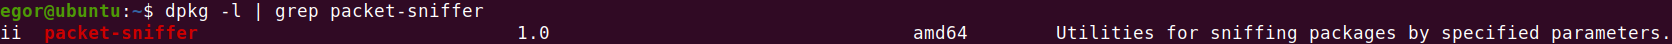
\includegraphics[scale=0.32]{../assets/check.png}
\end{center}

\subsubsection*{Удаление}

\begin{lstlisting}
$ make clean
\end{lstlisting}
или
\begin{lstlisting}
$ sudo dpkg -r packet-sniffer
\end{lstlisting}
